\documentclass[12pt]{article}
\usepackage{float}
\usepackage[table,xcdraw]{xcolor}
\usepackage{tikzit}
\input{Homework.tikzstyles}
\usepackage{hyperref}
\usepackage{amsmath}
\usepackage{amsfonts}
\usepackage{amssymb}
\usepackage{amsthm}
\usepackage{graphics}
\usepackage{graphicx}
\usepackage{yfonts}
\usepackage{float}
\usepackage[textwidth=17cm, textheight=24cm]{geometry}
\usepackage{dsfont}
\usepackage[nottoc]{tocbibind}
\setcounter{tocdepth}{3}
\setcounter{secnumdepth}{3}
\usepackage{url}
\usetikzlibrary{positioning}
\usepackage{neuralnetwork} 
\usepackage{multirow}
\usepackage{subcaption}
\usepackage{caption}
\usepackage[font=scriptsize]{caption}
\usepackage{ctable}
\usepackage{caption}
\usepackage{pifont}
\usepackage{array}
\usepackage{multirow}
\usepackage{subcaption}
\usepackage{ctable}
\usepackage{adjustbox}
\usepackage{booktabs}
\usepackage{tabularx, booktabs, makecell, caption}
\usepackage{siunitx}
\usepackage{booktabs}
\usepackage{xepersian}
\settextfont[
BoldFont=XB ZarBd.TTF,
ItalicFont=XB ZarIt.TTF,
BoldItalicFont=XB ZarBdIt.TTF]{XB Zar.TTF}
\ExplSyntaxOn \cs_set_eq:NN \etex_iffontchar:D \tex_iffontchar:D \ExplSyntaxOff
\setdigitfont[
BoldFont=XB ZarBd.TTF,
ItalicFont=XB ZarIt.TTF,
BoldItalicFont=XB ZarBdIt.TTF]{XB Zar.TTF}

\title{\Large پروژه سوم درس علوم اعصاب محاسباتی\\[1ex]آشنایی با انواع روش‌های کدگذاری و روش‌های یادگیری بدون ناظر و تقویتی}
\author{\\ \Large{ محمد زمانی}  \\ \\ \Large{شماره دانشجویی: ۶۱۰۳۹۹۱۳۵} \\ \\ }}
\date{}

\usepackage{titling}
\renewcommand\maketitlehooka{\null\mbox{}\vfill}
\renewcommand\maketitlehookd{\vfill\null}

\begin{document}
	%%%%%%%%%%%%%%%%%%%%%       Title Page      %%%%%%%%%%%%%%%%%%%%%%		

	
	\begin{titlingpage}
	
	\begin{figure}
		\centering
		
\includegraphics[width=0.3\textwidth]{Figs/University_of_Tehran_logo.png}	
		\caption*{ \LARGE دانشگاه تهران\\ دانشکده ریاضی و علوم کامپیوتر \\}
	\end{figure}	\maketitle
	
	\end{titlingpage}

	%%%%%%%%%%%%%%%%%%%%%       Page 1       %%%%%%%%%%%%%%%%%%%%%%

	\setlength{\parindent}{20pt}
	\tableofcontents
	
	\vspace{1\baselineskip}

	\pagebreak
	\section{مقدمه}
تا به اینجای کار ما انواع مدل‌های نورونی را مورد بررسی قرار دادیم و سپس جمعیت‌های نورونی و ارتباطات میان‌ آن‌ها را شبیه سازی کردیم و رفتار آن‌ها را در شرایط مختلف تحلیل کردیم. حال قصد داریم که فرآیند‌های کدگذاری در هنگام ورودی دادن به شبکه را شبیه سازی کنیم و سپس می‌خواهیم ببینیم که چگونه شبکه ما یاد خواهد گرفت و آن را شبیه سازی خواهیم کرد و تحلیل می‌کنیم.

	\section{کدگذاری}
	
	\subsection{\lr{ Time To First Spike}}
	
	در روش کدگذاری \lr{TTFS} ما به دنبال زمانی هستیم که نورون اولین ضربه خود را می‌زند، به عبارت دیگر از لحظه‌ای که ورودی به نورون داده می‌شود تا زمانی که نورون ضربه می‌زند را به عنوان چیزی که اطلاعات در آن وجود دارد ذخیره و کد می‌کنیم. که شماتیک کلی آن را می‌توانید در شکل \ref{Fig:ttfs} مشاهده کنید.

\begin{figure}[H]
\centering
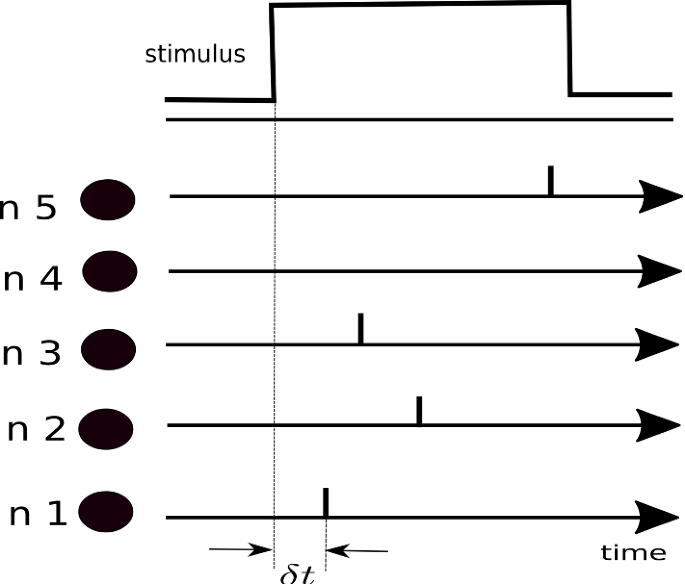
\includegraphics[width=4.5cm]{Figs/ttfs.png}
\caption{\lr{Time To First Spike}}
\label{Fig:ttfs}
\end{figure}
\end{center}

حال برای پیاده سازی این روش ما ورودی‌‌ها را نرمال می‌کنیم در یک بازه مثل صفر تا یک و یک پارامتر $T$
داریم، این بازه صفر تا یک را به $T$ قسمت مساوی تقسیم خواهیم کرد و با توجه به اینکه ورودی در بازه چندم قرار می‌گیرد در آن زمان ضربه خواهد زد، شکل \ref{Fig:int}.


\begin{figure}[H]
\centering
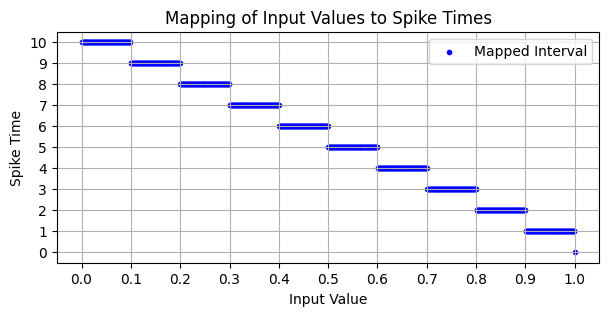
\includegraphics[width=7cm]{Figs/interval.png}
\caption{نحوه شبیه‌سازی \lr{Time To First Spike}}
\label{Fig:int}
\end{figure}
\end{center}

حال با استفاده از کدگذاری پیاده شده چهار عکس متفاوت را هم به صورت اورجینال هم به صورت فشرده شده کدگذاری می‌کنیم و می‌توانید نتایج آن و \lr{raster plot} را در شکل \ref{Fig:ttfs_res} مشاهده کنید.

\begin{figure}[H]
\centering
  \begin{subfigure}[b]{0.45\textwidth}
    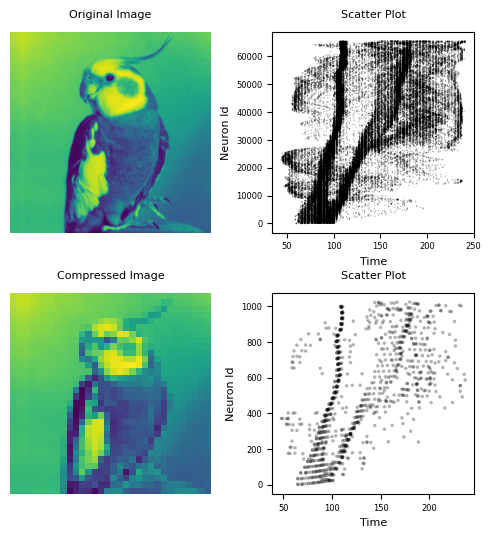
\includegraphics[width=\textwidth]{Figs/ttfs_bird.png}
  \end{subfigure}
  \hfill
  \begin{subfigure}[b]{0.45\textwidth}
    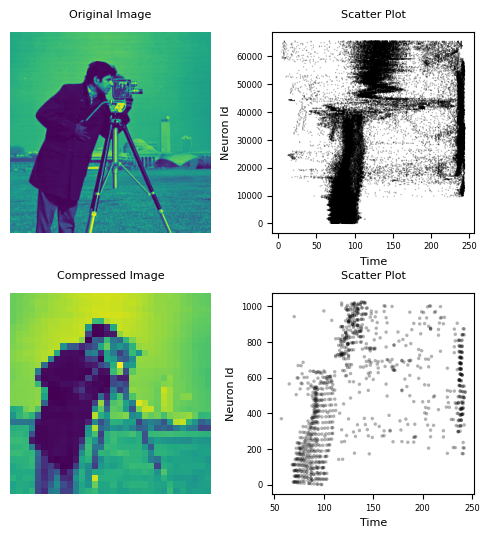
\includegraphics[width=\textwidth]{Figs/ttfs_cam.png}
  \end{subfigure}
  \\[\smallskipamount]
  \begin{subfigure}[b]{0.45\textwidth}
    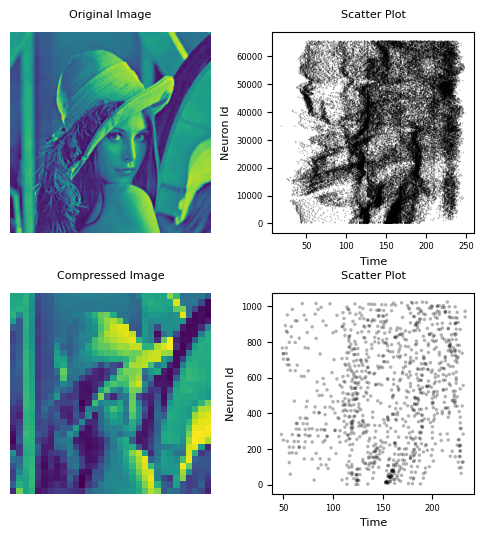
\includegraphics[width=\textwidth]{Figs/ttfs_lena.png}
  \end{subfigure}
  \hfill
  \begin{subfigure}[b]{0.45\textwidth}
    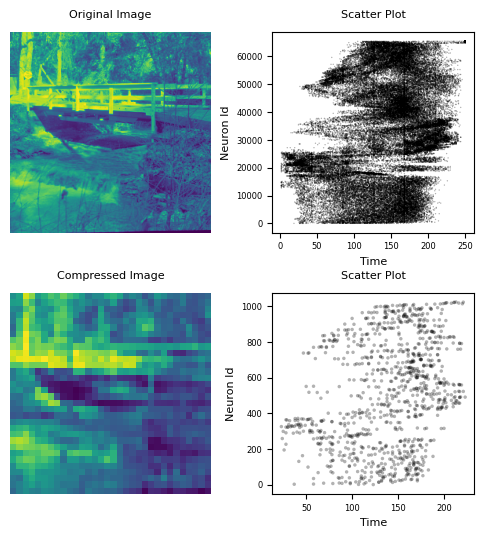
\includegraphics[width=\textwidth]{Figs/ttfs_bridge.png}
  \end{subfigure}
  \caption{\lr{raster plot} برای ضربه‌های تولید شده با استفاده از روش کدگذاری \lr{TTFS}}
  \label{Fig:ttfs_res}
\end{figure}
\end{center}

	\subsection{کدگذاری مقادیر عددی}
	
	در این روش بازه ۰ تا ۲۵۵ را که ورودی ما در این بازه قرار دارد به $T$	قسمت مساوی تقسیم  می‌کنیم که این $T$ یک پارامتر است، سپس توزیع‌های نرمالی با میانگین هایی که در این تقسیم بندی بدست آوردیم با یک انحراف معیار ثابت که پارامتر ما است رسم می‌کنیم، حال برای هر ورودی ما نقاط تلاقی آن نقطه با این توزیع‌ها را به عنوان زمان ضربه نورون در نظر می‌گیریم، به این صورت برای هر ورودی می‌توانیم یک دنباله‌ای از ضربه‌ها به صورت کد شده ارائه دهیم، شکل \ref{Fig:ac}.


\begin{figure}[H]
\centering
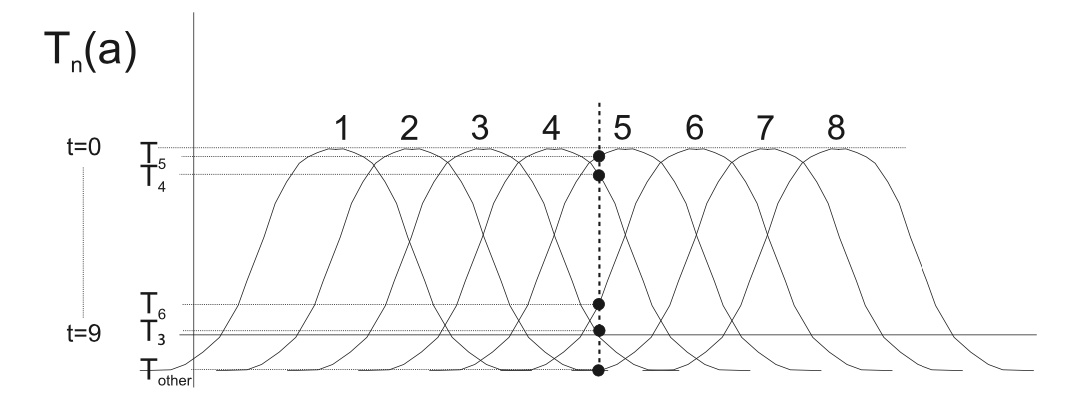
\includegraphics[width=7cm]{Figs/nc}
\caption{کدگذاری مقادیر عددی}
\label{Fig:ac}
\end{figure}
\end{center}


حال با توجه به توضیحات داده شده مانند قسمت قبل ورودی‌ها را در مدت زمان $T = 100ms$ ورودی می‌دهیم و \lr{raster plot}
حاصل را می‌توانید در شکل \ref{Fig:ac_res} مشاهده کنید.


\begin{figure}[H]
\centering
  \begin{subfigure}[b]{0.45\textwidth}
    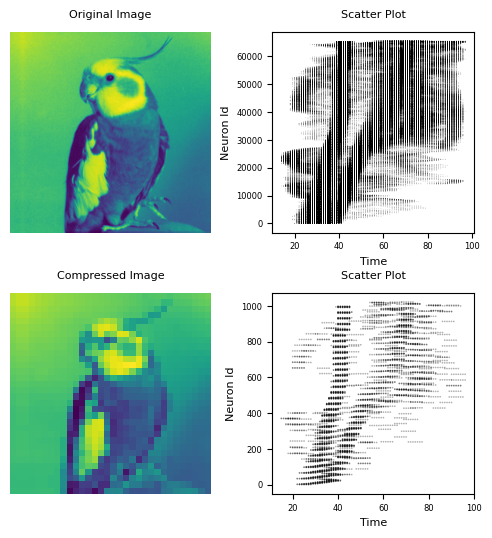
\includegraphics[width=\textwidth]{Figs/nc_bird.png}
  \end{subfigure}
  \hfill
  \begin{subfigure}[b]{0.45\textwidth}
    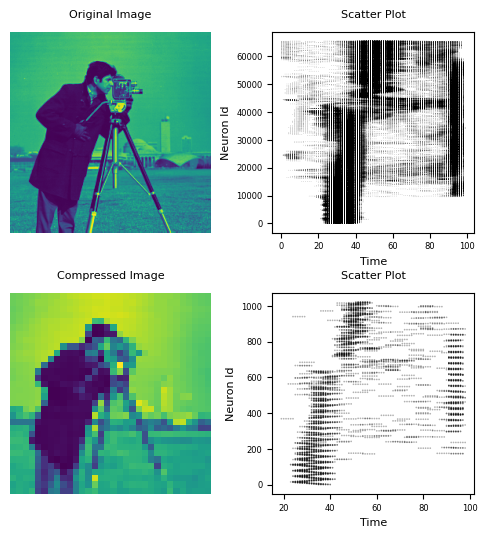
\includegraphics[width=\textwidth]{Figs/nc_cam.png}
  \end{subfigure}
  \\[\smallskipamount]
  \begin{subfigure}[b]{0.45\textwidth}
    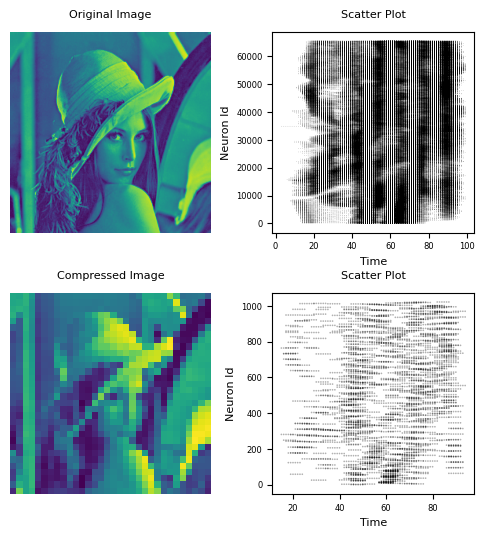
\includegraphics[width=\textwidth]{Figs/nc_lena.png}
  \end{subfigure}
  \hfill
  \begin{subfigure}[b]{0.45\textwidth}
    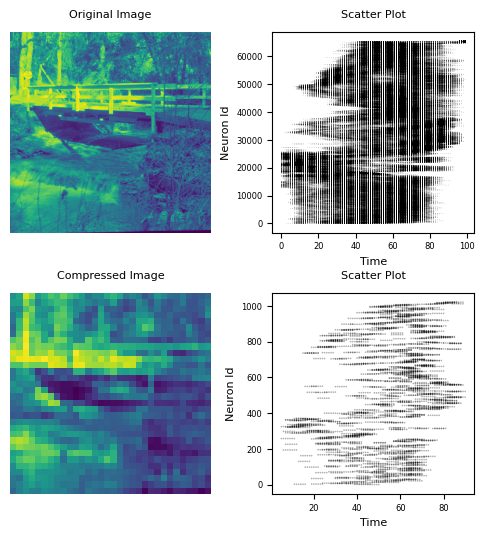
\includegraphics[width=\textwidth]{Figs/nc_bridge.png}
  \end{subfigure}
  \caption{\lr{raster plot} برای ضربه‌های تولید شده با استفاده از روش کدگذاری مقادیر عددی}
  \label{Fig:ac_res}
\end{figure}
\end{center}


\subsection{کدگذاری به کمک توزیع پوآسون}

در این روش از کدگذاری زمان میان ضربه‌های تولید شده را با استفاده از توزیع پوآسون بدست می‌اوریم، شکل توزیع پوآسون را می‌توانید در شکل \ref{Fig:p-d} مشاهده کنید، همانطور که می‌بنید در این توزیع یک پارامتر به نام $\lambda$ نیز وجد دارد که ما آن را در آزمایشمان $0.09$ قرار دادیم. در نهایت مانند قسمت‌های قبل ورودی را  در مدت زمان $T = 60ms$ ورودی دادیم و نتیجه را می‌توانید در شکل \ref{Fig:pc_res} مشاهده کنید.


\begin{figure}[H]
\centering
  \begin{subfigure}[b]{0.45\textwidth}
    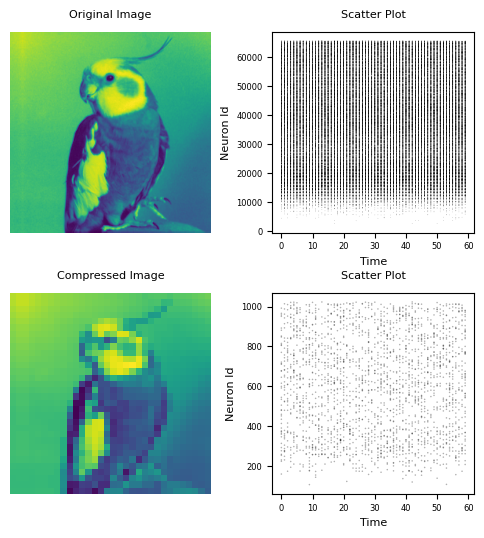
\includegraphics[width=\textwidth]{Figs/p_bird.png}
  \end{subfigure}
  \hfill
  \begin{subfigure}[b]{0.45\textwidth}
    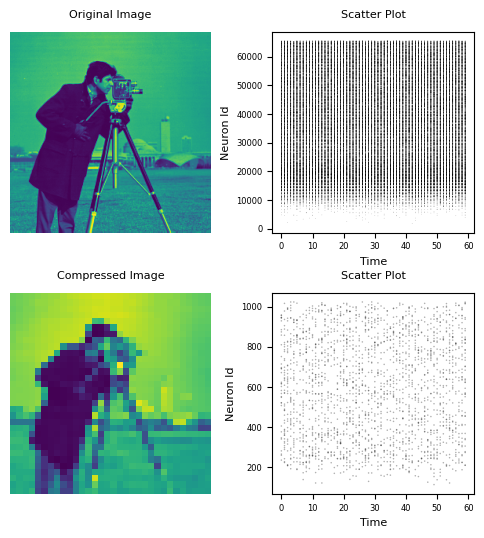
\includegraphics[width=\textwidth]{Figs/p_cam.png}
  \end{subfigure}
  \\[\smallskipamount]
  \begin{subfigure}[b]{0.45\textwidth}
    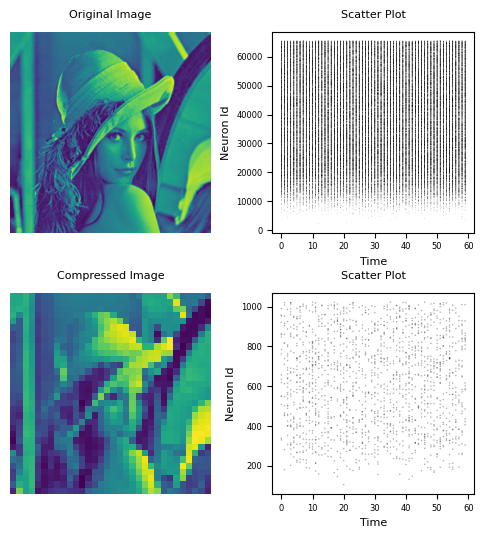
\includegraphics[width=\textwidth]{Figs/p_lena.png}
  \end{subfigure}
  \hfill
  \begin{subfigure}[b]{0.45\textwidth}
    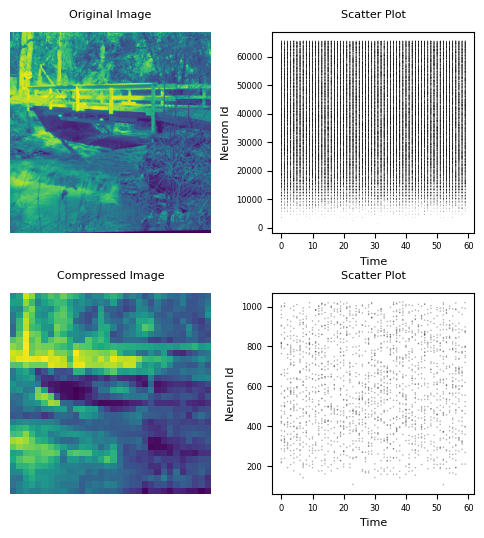
\includegraphics[width=\textwidth]{Figs/p_bridge.png}
  \end{subfigure}
  \caption{\lr{raster plot} برای ضربه‌های تولید شده با استفاده از روش کدگذاری به کمک توزیع پوآسون}
  \label{Fig:pc_res}
\end{figure}
\end{center}


\begin{figure}[H]
\centering
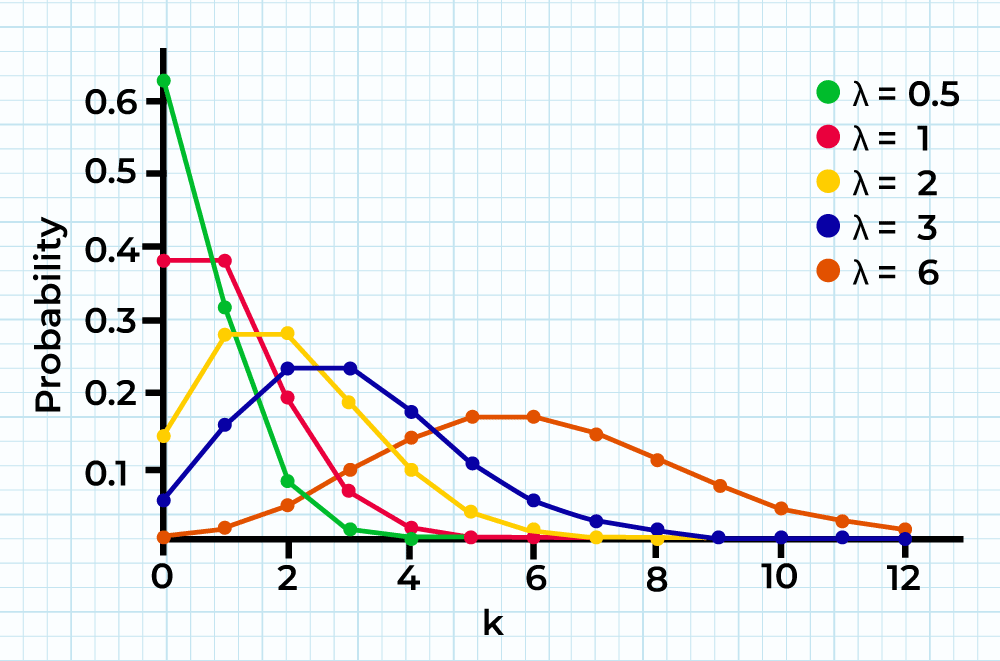
\includegraphics[width=9cm]{Figs/p-d.png}
\caption{توزیع پوآسون}
\label{Fig:p-d}
\end{figure}
\end{center}


در اینجا در توزیع پوآسون پارامتر $\lambda$ در واقع نشان دهنده نسبت یا میزان ضربه‌ها می‌باشد که هر چه آن را عدد بزرگتری قرار دهیم تعداد ضربه‌هایی که نورون می‌زند بیشتر خواهد شد زیرا با افزایش مقدار $\lambda$ مقدار شانس ضربه را افزایش می دهیم، به عنوان مثال برای تصویر پرنده این آزمایش را با مقادیر مختلف $\lambda$ تست می‌کنیم و نتیجه آن را می‌تواند در شکل \ref{Fig:lambda_res} مشاهده کنید.


\begin{figure}[H]
\centering
  \begin{subfigure}[b]{0.35\textwidth}
    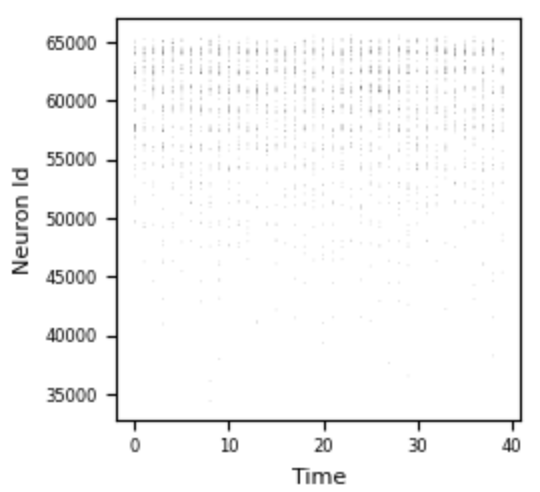
\includegraphics[width=\textwidth]{Figs/1}
    \caption{$\lambda = 0.03$}
  \end{subfigure}
  \hspace*{50}
  \begin{subfigure}[b]{0.35\textwidth}
    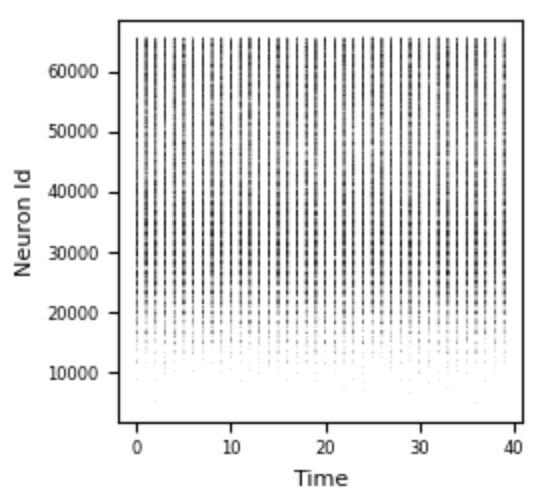
\includegraphics[width=\textwidth]{Figs/2}
    \caption{$\lambda = 0.08$}
  \end{subfigure}
  \\[\smallskipamount]
  \begin{subfigure}[b]{0.35\textwidth}
    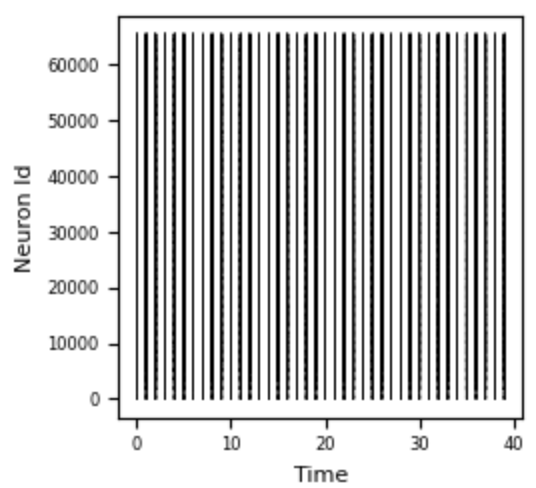
\includegraphics[width=\textwidth]{Figs/3}
    \caption{$\lambda = 0.5$}
  \end{subfigure}
  \hspace*{50}
  \begin{subfigure}[b]{0.35\textwidth}
    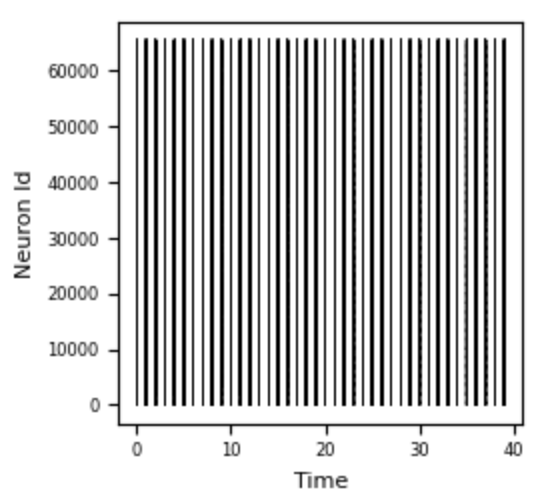
\includegraphics[width=\textwidth]{Figs/4}
    \caption{$\lambda = 1.0$}
  \end{subfigure}
  \caption{نقش پارامتر $\lambda$ در میزان ضربه‌های نورون}
  \label{Fig:lambda_res}
\end{figure}
\end{center}



\section{یادگیری بدون ناظر \lr{STDP}}

\subsection{\lr{STDP}}

اگر که ما دو الکترود داشته باشیم به طوری که الکترودها درون غشای نورونی قرار گیرند و از یکی از آن‌ها برای تحریک نورون استفاده کنیم و از دیگری برای اندازه گیری \lr{Neuron Response} استفاده کنیم، می‌توانیم مشاهده کنیم که اگر که نورون قبلی فعال شود و سپس با یک فاصله زمانی کوتاهی نورون بعدی متصل به قبلی فعال شود قدرت سیناپسی میان این دو نورون بیشتر می‌شود که این نشان می‌دهد تغییر وزن سیناپسی می‌تواند تابعی از 
$ t_j^f - t_i^f $
باشد.
 
 
\begin{figure}[H]
\centering
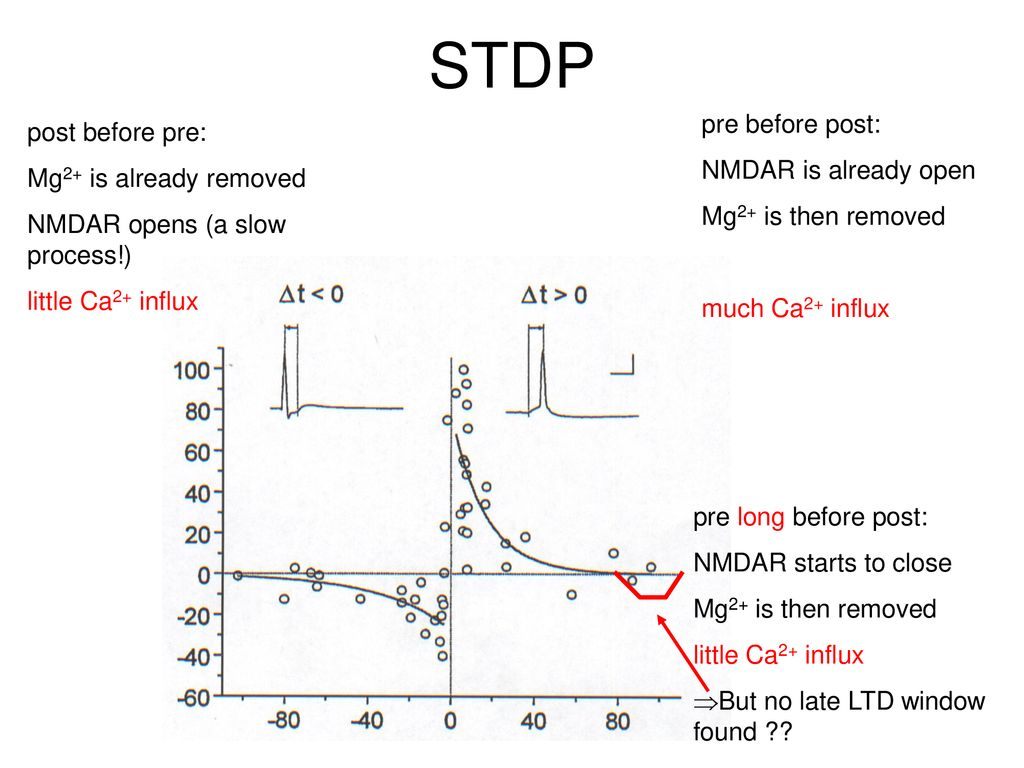
\includegraphics[width=9cm]{Figs/STDP.jpg}
\caption{فرآیند یادگیری \lr{STDP}, به فرآیند افزایش وزن در این قانون یادگیری \lr{LTP} و به فرآیند کاهش وزن \lr{LTD} می‌گویند.}
\label{Fig:p-d}
\end{figure}
\end{center}
 
 
 
 به طور کلی می‌توانیم تغییرات وزن بر حسب زمان را با این معادله شبیه سازی کنیم:
 
 $$ \frac{dw_{ij}}{dt} = -A_-(w_{ij})y_i(t)\Sigma_f \delta(t-t_j^f) + A_+(w_{ij})x_j(t)\Sigma_f \delta(t-t_i^f)$$
 
 
 \subsection{ساختار کلی شبکه}
 
برای انجام آزمایشات شبکه ما به طور کلی متشکل از سه جمعیت نورونی خواهد بود که که دو جمعیت نورونی متشکل از چهار نورون داریم که به یک جمعیت نورونی متشکل از دو نورون متصل هستند، در واقع این جمعیت دو نورونی نقش خروجی ‌های ما را دارند، ورودی ها نیز به دو جمعیت نورونی چهار نورونی داده می‌شود که این ساختار را می‌تواند در شکل \ref{Fig:inp}	مشاهده کنید.
 
\begin{figure}[H]
\centering
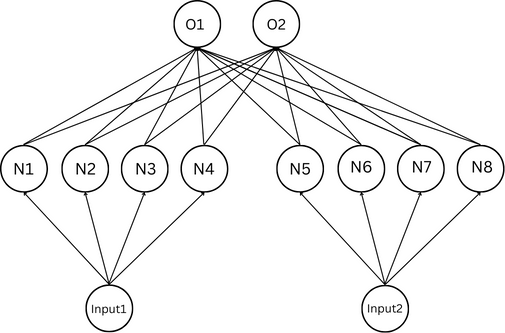
\includegraphics[width=7cm]{Figs/inputq.png}
\caption{ساختار شبکه ساخته شده}
\label{Fig:inp}
\end{figure}
\end{center}


\subsection{ورودی‌های شبکه}

\subsubsection{جریان ثابت با نویز}
در این حالت به هر یک از جمعیت‌های نورونی چهار نورونی یک جریان مجزا وارد می‌کنیم، این جریان یک مقدار ثابت خواهد داشت که به آن مقدار ثابت با توزیع نرمال نویز وارد می‌کنیم.

به عنوان مثال به جمعیت نورونی اول جریان ثابت 200 با نویز وارد می‌کنیم و به جمعیت نورونی دوم جریان ثابت 50 با نویز وارد می‌کنیم که میتوانید نمودار جریان‌های ورودی و فعالیت شبکه را در شکل \ref{Fig:ng1-ng2-inp}
مشاهده کنید.


\begin{figure}[H]
\centering
  \begin{subfigure}[b]{0.9\textwidth}
    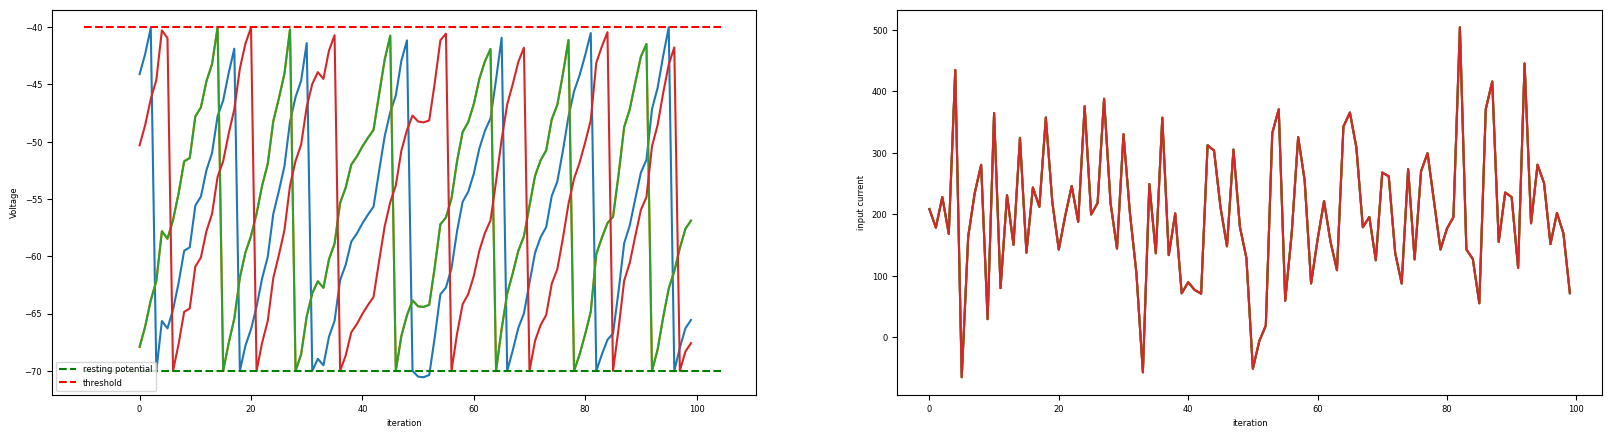
\includegraphics[width=\textwidth]{Figs/ng1-inp.png}
    \caption{جمعیت نورونی اول}
  \end{subfigure}
  \\[\smallskipamount]
  \begin{subfigure}[b]{0.9\textwidth}
    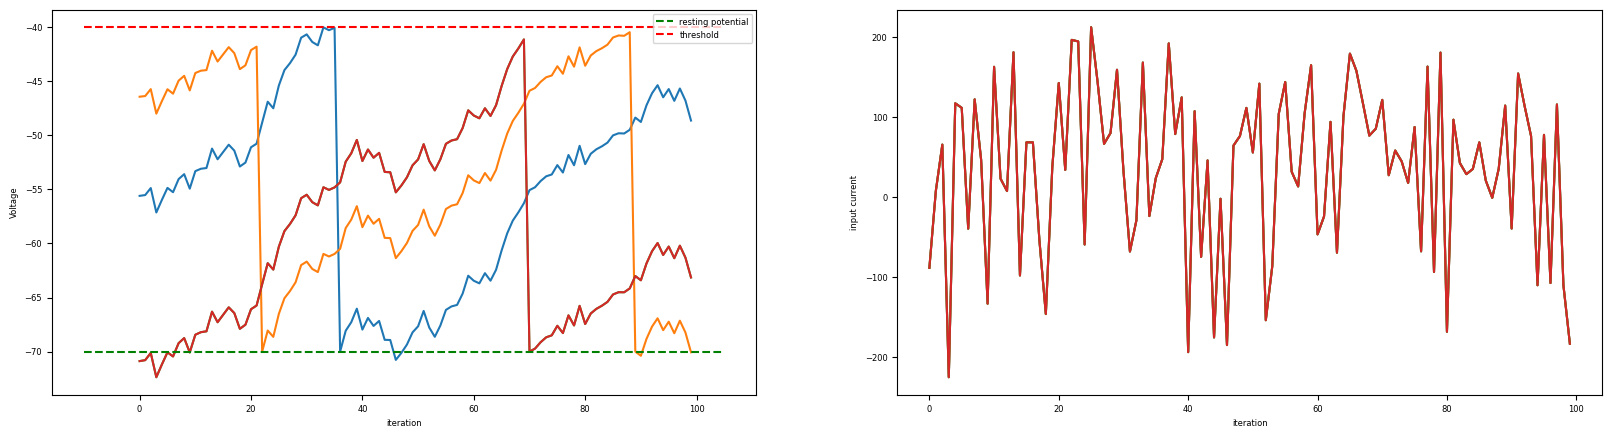
\includegraphics[width=\textwidth]{Figs/ng2-inp.png}
    \caption{جمعیت نورونی دوم}
  \end{subfigure}
  \caption{نمودار جریان ورودی و تغییرات پتانسیل نورون‌های جمعیت‌های نورونی}
  \label{Fig:ng1-ng2-inp}
\end{figure}
\end{center}


\begin{figure}[H]
\centering
  \begin{subfigure}[b]{0.30\textwidth}
    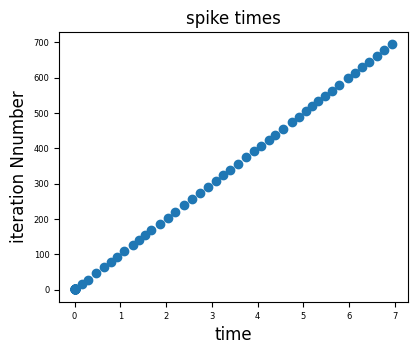
\includegraphics[width=\textwidth]{Figs/ng1-s-t.png}
    \caption{جمعیت نورونی اول}
  \end{subfigure}
  \hspace*{40}
  \begin{subfigure}[b]{0.30\textwidth}
    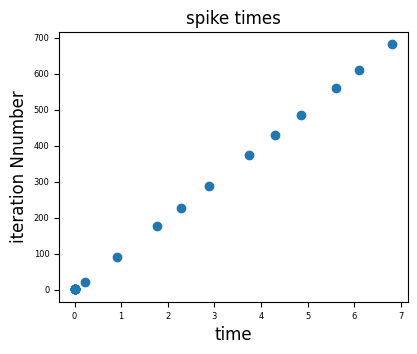
\includegraphics[width=\textwidth]{Figs/ng2-s-t.png}
    \caption{جمعیت نورونی دوم}
  \end{subfigure}
  \caption{نمودار زمان فعالیت جمعیت‌های نورونی}
  \label{Fig:s-t}
\end{figure}
\end{center}

\subsubsection{ورودی تصادفی با توزیع پوآسون}
در این قسمت از کدگذاری پوآسون که در بخش کدگذاری پوآسون توضیح دادیم استفاده می‌کنیم، یک عکس را انتخاب می‌کنیم و آن را کد می‌کنیم و ضربه‌های تولید شده را به عنوان ورودی به شبکه می‌دهیم و جمعیت نورونی را مجبور به آن رفتار می‌کنیم.

در این بخش از آزمایش ما دو عکس پرنده و پل انتخاب شده را به عنوان ورودی به دو جمعیت نورونی می‌دهیم به این صورت که به جمعیت اول ضربه‌های تولید شده توسط عکس پرنده و به جمعیت دوم ضربه‌های تولید شده توسط عکس پل را می‌دهیم، ضربه‌های این دو جمعیت نورونی را می‌توانید در شکل \ref{Fig:p-s-t} مشاهده کنید.


\begin{figure}[H]
\centering
  \begin{subfigure}[b]{0.30\textwidth}
    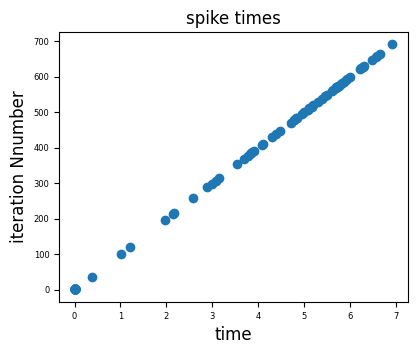
\includegraphics[width=\textwidth]{Figs/s-t-bird.png}
    \caption{جمعیت نورونی اول با ورودی پرنده}
  \end{subfigure}
  \hspace*{40}
  \begin{subfigure}[b]{0.30\textwidth}
    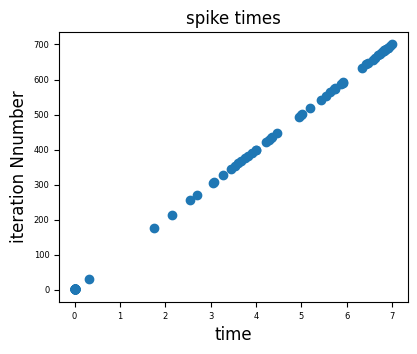
\includegraphics[width=\textwidth]{Figs/s-t-bridge.png}
    \caption{جمعیت نورونی دوم با ورودی پل}
  \end{subfigure}
  \caption{نمودار زمان فعالیت جمعیت‌های نورونی}
  \label{Fig:p-s-t}
\end{figure}
\end{center}



\subsection{تغییرات وزن سیناپسی}

اگر نورون‌های هر یک از جمعیت‌های نورونی را از یک تا $n$ شماره گذاری کنیم، $w_{ij}$ نشان دهنده وزن میان نورون $i$ام از جمعیت قبلی به نورون $j$ام جمعیت بعدی است. در این بخش می‌خواهیم تغییرات وزن سیناپسی را نشان دهیم.

\subsubsection{تغییرات وزن سیناپسی با جریان ثابت نویز دار}

\begin{figure}[H]
\centering
  \begin{subfigure}[b]{0.45\textwidth}
    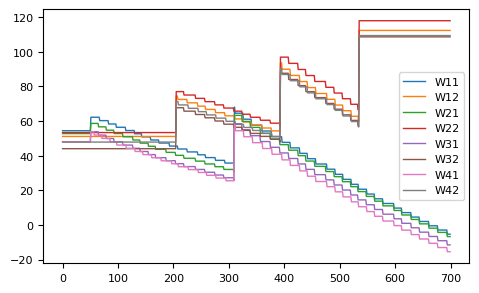
\includegraphics[width=\textwidth]{Figs/ng1-w.png}
    \caption{جمعیت نورونی اول}
  \end{subfigure}
  \hspace*{10}
  \begin{subfigure}[b]{0.45\textwidth}
    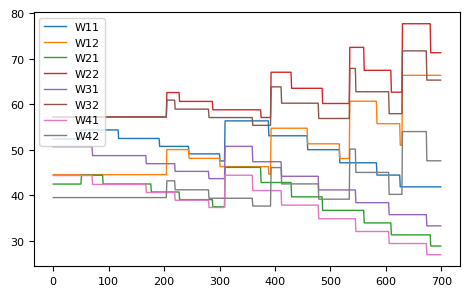
\includegraphics[width=\textwidth]{Figs/ng2-w.png}
    \caption{جمعیت نورونی دوم}
  \end{subfigure}
  \caption{نمودار تغییرات وزن‌های سیناپسی جمعیت‌های نورونی}
  \label{Fig:ng1-ng2-w}
\end{figure}
\end{center}

\begin{figure}[H]
\centering
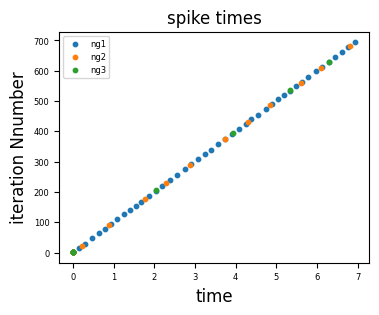
\includegraphics[width=7cm]{Figs/ngs-s-t.png}
\caption{زمان ضربه هر سه جمعیت نورونی موجود در شبکه}
\label{Fig:ngs-s-t}
\end{figure}
\end{center}

همانطور که در شکل \ref{Fig:ngs-s-t} مشاهده می‌کنید فواصل زمانی ضربه بین نورون‌های جمعیت اول با ضربه‌های جمعیت خروجی نسبت به جمعیت دوم و جمعیت خروجی کمتر می‌باشد و در نتیجه این مورد طبق تعریف قانون یادگیری $STDP$ باعث می‌شود که افزایش وزن در جکعیت اول بیشتر باشد و همچنین شدت کاهش وزن نیز بیشتر باشد.

\hfill \break
\subsubsection{تغییرات وزن سیناپسی با ورودی تصادفی پوآسون}

\begin{figure}[H]
\centering
  \begin{subfigure}[b]{0.45\textwidth}
    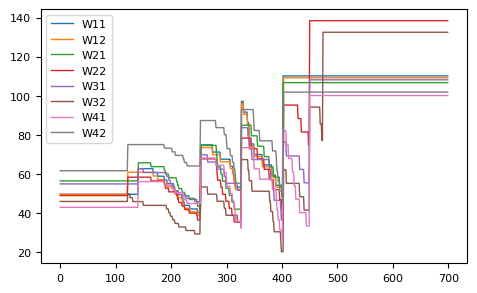
\includegraphics[width=\textwidth]{Figs/w-ng1.png}
    \caption{جمعیت نورونی اول با ورودی پرنده}
  \end{subfigure}
  \hspace*{10}
  \begin{subfigure}[b]{0.45\textwidth}
    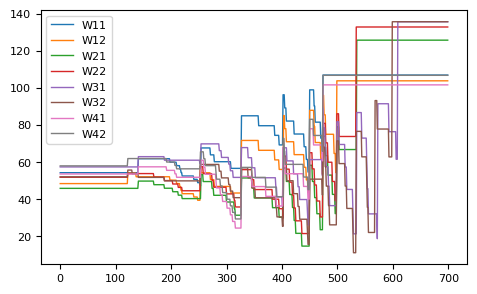
\includegraphics[width=\textwidth]{Figs/w-ng2.png}
    \caption{ جمعیت نورونی دوم با ورودی پل}
  \end{subfigure}
  \caption{نمودار تغییرات وزن‌های سیناپسی جمعیت‌های نورونی}
  \label{Fig:w-ng1-ng2}
\end{figure}
\end{center}

\begin{figure}[H]
\centering
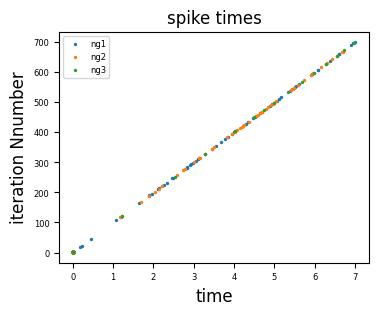
\includegraphics[width=7cm]{Figs/ngs-p-s-t.png}
\caption{زمان ضربه هر سه جمعیت نورونی موجود در شبکه}
\label{Fig:ngs-p-s-t}
\end{figure}
\end{center}

همانطور که مشاهده می‌کنید در این حالت که هر دو جمعیت نورونی ورودی ما ضربه‌هایی قبل از ضربه‌های جمعیت خروجی  داشتند باعث شده است که وزن‌های سیناپسی افزایش پیدا کنند، البته نکته مهمی که وجود دارد این است که ما برای کنترل افزایش وزن‌ها از \lr{hard bound} نیز استفاده کرده‌ایم که باعث می‌شود به وزن‌ها اجازه صعود بدون حد ندهد و این رفتار را در نمودارهای \ref{Fig:w-ng1-ng2}
می‌توانید مشاهده کنید.

\hfill \break
\subsection{شباهت کسینوسی}

\begin{figure}[H]
\centering
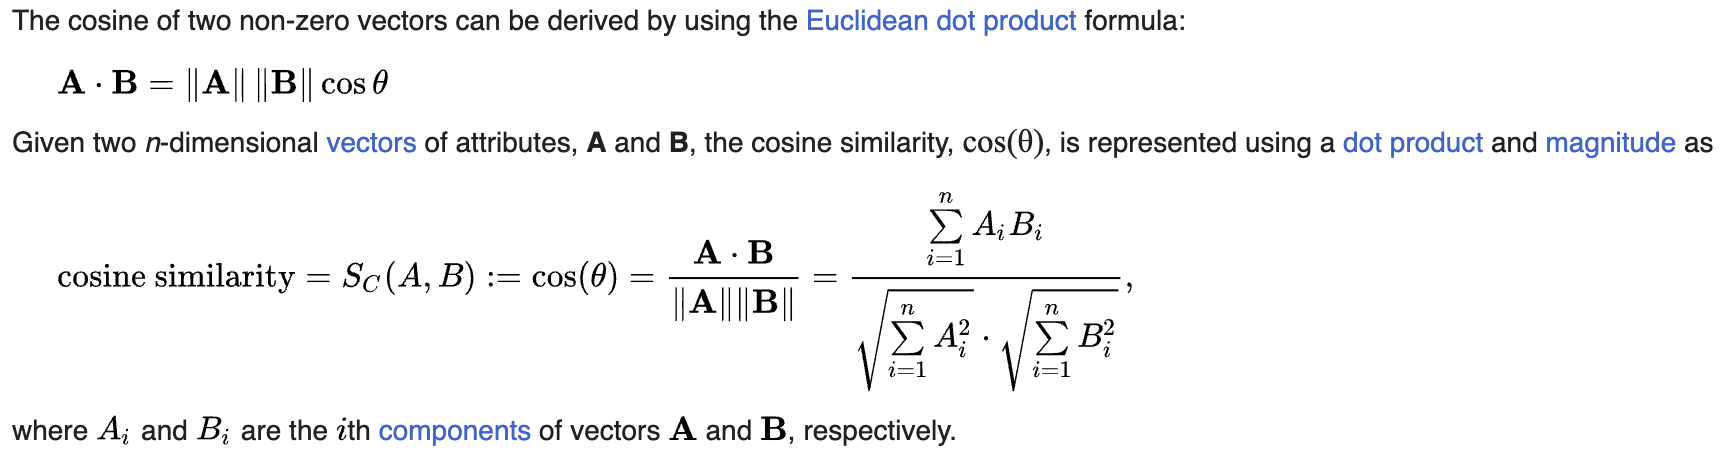
\includegraphics[width=17cm]{Figs/cos-sim-def}
\caption{تعریف شباهت کسینوسی}
\label{Fig:cos-sim-def}
\end{figure}
\end{center}

همانطور که در شکل \ref{Fig:inp} نشان داده شده است، به هر نورون خروجی هشت نورون متصل است که این به معنای وجود هشت وزن سیناپسی می‌باشد، حال برای هر مرحله از شبیه سازی برای هر نورون خروجی یک بردار هشت تایی از وزن‌ها در آن لحظه خواهیم داشت که می‌توانیم برای این بردار ها شباهت کسینوسی را اندازه گیری کنیم.

\hfill \break
\subsubsection{شباهت کسینوسی با جریان ثابت نویز دار}

همانطور که بالاتر توضیح دادیم در این قسمت شباهات کسینوسی را در هر مرحله از شبیه سازی محاسبه می‌کنیم که نتیجه آن را  در نمودار \ref{Fig:cos-sim}	می‌توانید مشاهده کنید. 

\begin{figure}[H]
\centering
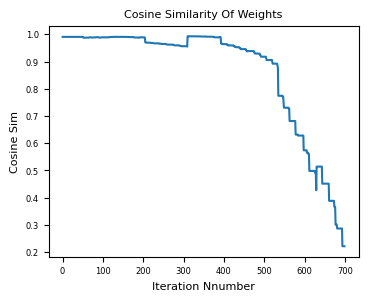
\includegraphics[width=6cm]{Figs/cos-sim.png}
\caption{نمودار  شباهت کسینوسی وزن‌های دو نورون خروجی}
\label{Fig:cos-sim}
\end{figure}
\end{center}



اگر که وظیفه ما یک $classification$ باشد در آن زمان هر نورون خروجی ما بازنمایی یک کلاس خواهد بود، بنابراین زمانی این مدل به خوبی عمل می‌کند که شباهت میان این نورون‌های خروجی به کمینه خود برسند چون کاملا در این صورت الگوهای متفاوتی را آموخته‌اند، در اینجا هم همانطور که مشاهده می‌کنید به مرور زمان وقتی شبیه سازی را انجام می‌دهیم شباهت میان وزن‌ها کمتر می‌شود که این نشان دهنده یادگیری الگو‌های متفاوت توسط نورون‌های خروجی می‌باشد که این مطابق انتظار ما رفتار خوبی است چونکه ما دوجمعیت با ورودی‌های کاملا متفاوت داشتیم و انتظار داشتیم که بتوانیم تفاوت‌ آن‌ها را در نورون‌های خارجی نیز مشاهده کنیم.



\subsubsection{شباهت کسینوسی با ورودی تصادفی پوآسون}
همانطور که ابندای این بخش توضیح دادیم در این قسمت شباهات کسینوسی را در هر مرحله از شبیه سازی محاسبه می‌کنیم که نتیجه آن را  در نمودار \ref{Fig:cos-sim2}	می‌توانید مشاهده کنید. 


\begin{figure}[H]
\centering
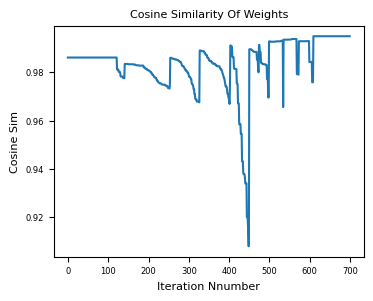
\includegraphics[width=6cm]{Figs/cos-sim2.png}
\caption{نمودار  شباهت کسینوسی وزن‌های دو نورون خروجی}
\label{Fig:cos-sim2}
\end{figure}
\end{center}

اگر که وظیفه ما یک $classification$ باشد وقتی می‌توانیم به خوبی عمل کنیم که شباهت به میزان کمینه خود برسد و این البته در حالتی خوب است که الگو‌های ورودی هم کاملا متفاوت باشند، برای مثال در بخش ورودی با جریان ثابت نویز دار که الگو ها تفاوت زیادی داشتند این شباهت خیلی کم بود و نورون‌های خروجی رفتار های متفاوتی را آموختند اما در این بخش همانطور که در شکل \ref{Fig:cos-sim2}
مشاهده می‌کنید نورون‌های خروجی ما الگو‌های خیلی متفاوتی را نیاموخته‌اند و تقریبا می‌توان گفت که الگو ها با هم مشابه بوده‌اند اما با این حال می‌توان از آن‌ها برای جداسازی کلاس ها استفاده کرد.

\subsection{تاثیر نورون بدون فعالیت}

در این بخش یک جمعیت نورونی با یک  نورون به دو جمعیت نورونی ورودی اضافه می‌کنیم که به آن ورودی نمی‌دهیم تا ضربه ای نزند همچنین یک جمعیت نورونی نیز به خروجی اضافه می‌کنیم که در آن نیز با افزایش حد آستانه کاری می‌کنیم که آن نورون ضربه ای نزند، بنابراین در این شبکه جدید نه نورون در لایه ورودی داریم که از سه جمعیت تشکیل شده اند و دو جمعیت در لایه خروجی داریم که در کل سه نورون دارند. 
\subsubsection{تاثیر نورون بدون فعالیت با جریان ورودی ثابت نویزدار}

در این حالت از آنجایی که نورون خروجی‌ای که اضافه کردیم هیچ ضربه ای نمی‌زند بنابراین وزن سیناپسی متصل به آن نورون نیز تغییری ندارد، ما نه نورون متصل به این نورون داریم که تغییرات وزن های سیناپسی را می‌توانید در شکل 
\ref{Fig:out_plus}
مشاهده کنید و همانطور که می‌بینید تغییری مشاهده نمی‌شود.

\begin{figure}[H]
\centering
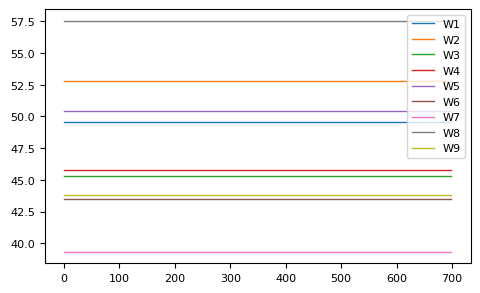
\includegraphics[width=6cm]{Figs/out_plus.png}
\caption{تغییر وزن‌های سیناپسی نورون بدون فعالیت خروجی}
\label{Fig:out_plus}
\end{figure}
\end{center}


\subsubsection{تاثیر نورون بدون فعالیت با ورودی تصادفی پوآسون}

همانطور که در قسمت قبلی توضیح داده شد از آنجایی که هیچ ضربه ای این نورون خروجی اضافه شده نمی‌زند بنابراین طبق تعریف قانون یادگیری \lr{STDP} هیچ تغییری در وزن‌های سیناپسی متصل به این نورون رخ نمی‌دهد و این موضوع را می‌توانید در شکل \ref{Fig:last-w-ch} مشاهده کنید.

\begin{figure}[H]
\centering
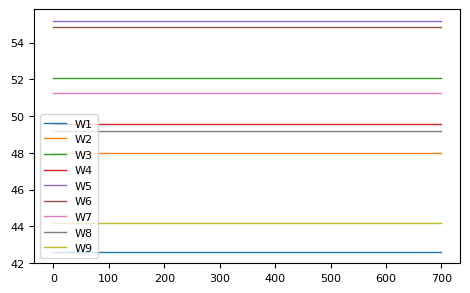
\includegraphics[width=6cm]{Figs/last-w-ch.png}
\caption{تغییر وزن‌های سیناپسی نورون بدون فعالیت خروجی}
\label{Fig:last-w-ch}
\end{figure}
\end{center}


\subsection{بررسی پارامتر‌های مهم}

از مهمترین پارامتر‌هایی که در این یادگیری موثر هستند می‌توان به این پارامترها اشاره کرده:


\subsubsection{$a_+$ و $a_-$}

این دو هر کدام ضرایبی برای افزایش و کاهش وزن می‌باشد که هر چه برای مثال $a_+$ را افزایش دهیم سرعت افزایش وزن‌ها بیشتر می‌شود و اگر $a_-$ را افزایش دهیم سرعت کاهش وزن افزایش می‌یابد. در آزمایشات انجام شده ما $a_-=a_+=2$
قرار داده‌ایم.

\subsubsection{محدودیت‌های وزنی}

در کل می‌توانیم از محدودیت های وزنی متفاوتی برای کنترل وزن‌ها استفاده کنیم که هر کدام از این روش‌ها نیز پارامترهای خاص خود را دارند، برای مثال در این آزمایشات ذکر شده از \lr{hard bound} استفاده کردیم و بیشینه وزن را مقدار $100$ قرار دادیم اما می‌توان آن را تغییر داد و از پارامترهای متفاوت دیگری استفاده کرد، از آنجایی که این پارامتر مفهوم خاصی ندارد و فقط برای کنترل وزن‌ها می‌باشد آن را با پارامتر دیگری تست نمی‌کنیم.


\section{یادگیری تقویتی \lr{RSTDP}}

\subsection{\lr{RSTDP}}
در یادگیری بدون ناظر \lr{STDP} ما کنترلی بر روند یادگیری نداریم و ماهیت این نوع یادگیری به این صورت است که چیزی که تکرار می‌‌شود و فرکانس آن زیاد است تقویت می‌شود و یادگرفته می‌شود اما در یادگیری تقویتی ما به دنبال این هستیم که با دادن مجازات و پاداش بر روی روند یادگیری کنترل داشته باشیم و در انتهای یادگیری کارهایی که منجرب پاداش می‌شوند را یاد بگیریم و از طرفی از کارهایی که منجرب مجازات می‌شوند دوری کنیم.

به نظر می‌رسد درون مغز ما یادگیری تقویتی به کمک ترشح دوپامین \LTRfootnote{Dopamine} در مغز انجام می‌شود، دوپامین یک \lr{Neuro-modulator} است که دورن مغز وجود دارد و بر روی روند یادگیری مغز نقش دارد. مطالعات نشان می‌دهد که زمانی که ما کاری انجام می‌دهیم که برای ما پاداشی به همراه دارد غلظت دوپامین در مغز ما بیشتر می‌شود و در صورتی که کار ما باعث مجازات شود غلظت دوپامین کم می‌شود. 


یکی از مسائل مهمی که در این نوع یادگیری با آن مواجه هستیم مسئله \lr{distal problem} است، وقتی که ما کاری انجام می‌دهیم ممکن است پس مدتی مجازات یا پاداش آن را دریافت کنیم بنابراین تشخیص اینکه هر پاداش مربوط به چه واکنشی بوده است بسیار مهم است.

آزمایشات نشان می‌دهند که دوپامین به دو صورت می‌تواند بر روی \lr{STDP} تاثیر بگذارد:

\begin{itemize}

\item[•] \lr{changing STDP's window}
\item[•] \lr{changing STDP's polarity}

\end{itemize}

اگر به هر کدام از این موارد یک متغیر نسبت دهیم آنگاه می‌توانیم دینامیک آن ها را به این صورت بیان کنیم:


$$ \frac{dc}{dt} = -\frac{c}{\tau_c} + STDP(I) \sigma(t - \frac{t_{pre}}{t_{post}}) $$

$$ \frac{ds}{dt} = c d $$

$$ \frac{dd}{dt} = -\frac{d}{\tau_d} + DA(t) $$


که $s$ نشان دهنده وزن سیناپسی است، $c$ نیز نشان دهنده همان فعالیت آهسته‌ای است که وقتی نورون قبلی فعال می‌شود و این فعالیت به نورون بعدی منتقل می‌شود، که در حین انجام این انتقال یک سری مکانیزم‌ها و \lr{path way} هایی فعال می‌شوند که به صورت لحظه‌ای نیستند و آهسته به وجود می‌آیند و آهسته از بین می‌روند، بنابراین $c$ به طور کلی فعالیت آنزیم‌هایی که در \lr{plasticity} مهم هستند را نشان می‌دهد. در نهایت $d$ نیز غلظت دوپامین را  نشان می‌دهد.



\subsection{ساختار کلی شبکه}
در این بخش نیز شبکه ما همانطور که در شکل \ref{Fig:inp}
نشان دادیم خواهد بود از سه جمعیت نورونی تشکیل شده است.

\subsection{ورودی‌های شبکه}

\subsubsection{جریان ثابت با نویز}
در این حالت به هر یک از جمعیت‌های نورونی چهار نورونی یک جریان مجزا وارد می‌کنیم، این جریان یک مقدار ثابت خواهد داشت که به آن مقدار ثابت با توزیع نرمال نویز وارد می‌کنیم.

به عنوان مثال به جمعیت نورونی اول جریان ثابت 200 با نویز وارد می‌کنیم و به جمعیت نورونی دوم جریان ثابت 50 با نویز وارد می‌کنیم که میتوانید نمودار جریان‌های ورودی و فعالیت شبکه را در شکل \ref{Fig:ng1-ng2-inp-r}
مشاهده کیند.


\begin{figure}[H]
\centering
  \begin{subfigure}[b]{0.9\textwidth}
    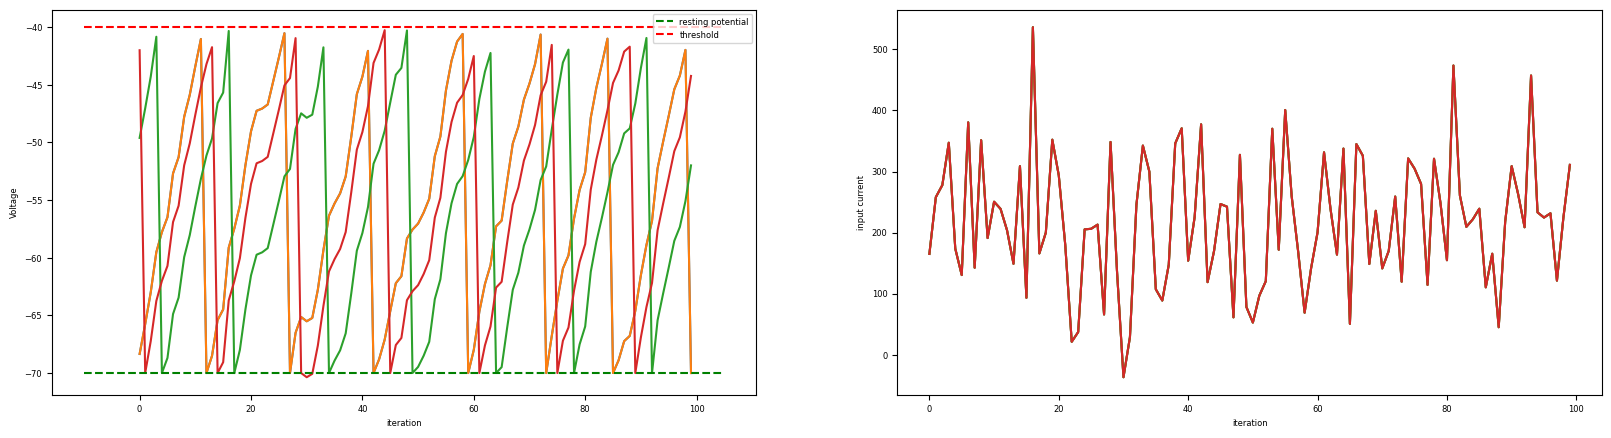
\includegraphics[width=\textwidth]{Figs/ng1-inp-r.png}
    \caption{جمعیت نورونی اول}
  \end{subfigure}
  \\[\smallskipamount]
  \begin{subfigure}[b]{0.9\textwidth}
    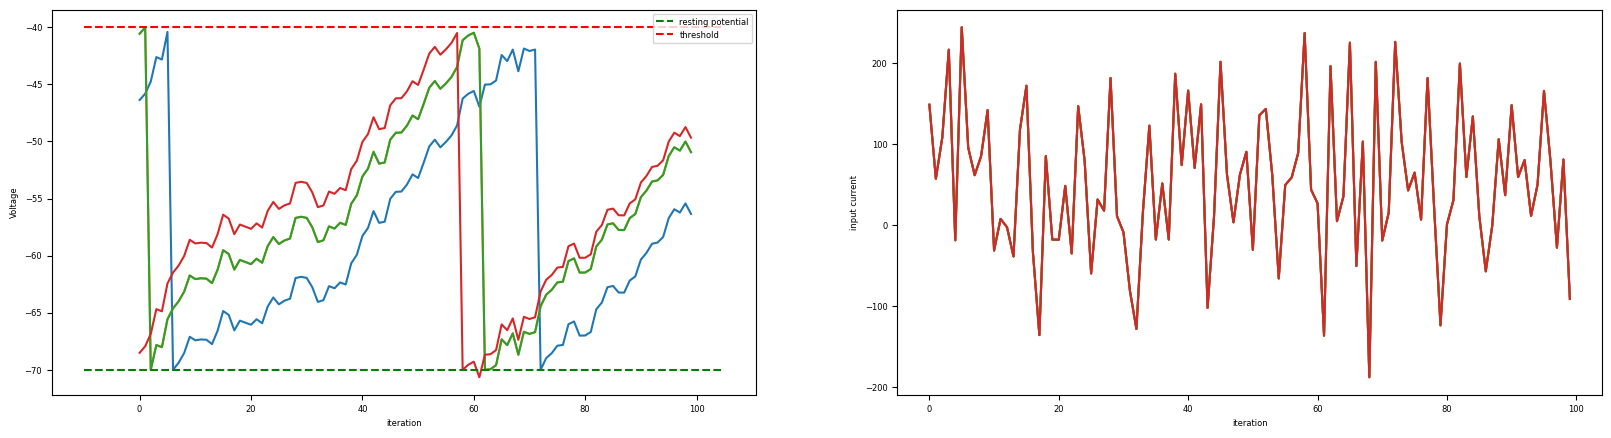
\includegraphics[width=\textwidth]{Figs/ng2-inp-r.png}
    \caption{جمعیت نورونی دوم}
  \end{subfigure}
  \caption{نمودار جریان ورودی و تغییرات پتانسیل نورون‌های جمعیت‌های نورونی}
  \label{Fig:ng1-ng2-inp-r}
\end{figure}
\end{center}


\begin{figure}[H]
\centering
  \begin{subfigure}[b]{0.30\textwidth}
    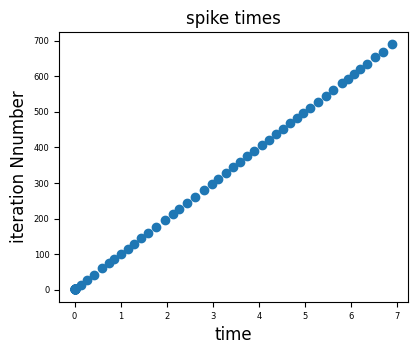
\includegraphics[width=\textwidth]{Figs/ng1-s-t-r.png}
    \caption{جمعیت نورونی اول}
  \end{subfigure}
  \hspace*{40}
  \begin{subfigure}[b]{0.30\textwidth}
    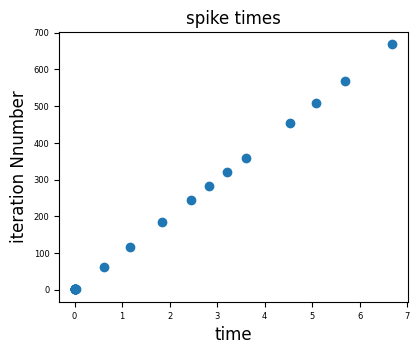
\includegraphics[width=\textwidth]{Figs/ng2-s-t-r.png}
    \caption{جمعیت نورونی دوم}
  \end{subfigure}
  \caption{نمودار زمان فعالیت جمعیت‌های نورونی}
  \label{Fig:s-t-r}
\end{figure}
\end{center}

\subsubsection{ورودی تصادفی با توزیع پوآسون}
در این قسمت از کدگذاری پوآسون که در بخش کدگذاری پوآسون توضیح دادیم استفاده می‌کنیم، یک عکس را انتخاب می‌کنیم و آن را کد می‌کنیم و ضربه‌های تولید شده را به عنوان ورودی به شبکه می‌دهیم و جمعیت نورونی را مجبور به آن رفتار می‌کنیم.

در این بخش از آزمایش ما دو عکس پرنده و پل انتخاب شده را به عنوان ورودی به دو جمعیت نورونی می‌دهیم به این صورت که به جمعیت اول ضربه‌های تولید شده توسط عکس پرنده و به جمعیت دوم ضربه‌های تولید شده توسط عکس پل را می‌دهیم، ضربه‌های این دو جمعیت نورونی را می‌توانید در شکل \ref{Fig:p-s-t-r} مشاهده کنید.


\begin{figure}[H]
\centering
  \begin{subfigure}[b]{0.30\textwidth}
    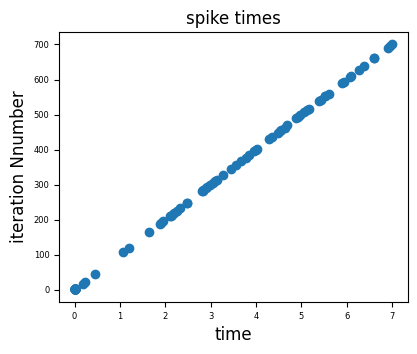
\includegraphics[width=\textwidth]{Figs/ng1-s-t-r2.png}
    \caption{جمعیت نورونی اول با ورودی پرنده}
  \end{subfigure}
  \hspace*{40}
  \begin{subfigure}[b]{0.30\textwidth}
    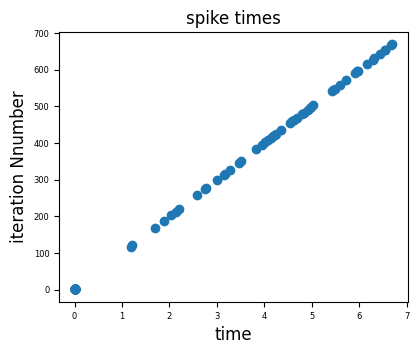
\includegraphics[width=\textwidth]{Figs/ng2-s-t-r2.png}
    \caption{جمعیت نورونی دوم با ورودی پل}
  \end{subfigure}
  \caption{نمودار زمان فعالیت جمعیت‌های نورونی}
  \label{Fig:p-s-t-r}
\end{figure}
\end{center}

\subsection{تغییرات وزن سیناپسی}
اگر نورون‌های هر یک از جمعیت‌های نورونی را از یک تا $n$ شماره گذاری کنیم، $w_{ij}$ نشان دهنده وزن میان نورون $i$ام از جمعیت قبلی به نورون $j$ام جمعیت بعدی است. در این بخش می‌خواهیم تغییرات وزن سیناپسی را نشان دهیم.

\subsubsection{تغییرات وزن سیناپسی با جریان ثابت نویز دار}

\begin{figure}[H]
\centering
  \begin{subfigure}[b]{0.45\textwidth}
    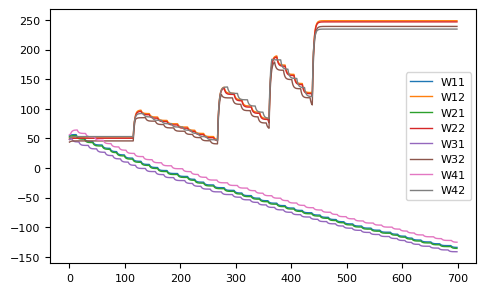
\includegraphics[width=\textwidth]{Figs/ng1-w-r.png}
    \caption{جمعیت نورونی اول}
  \end{subfigure}
  \hspace*{10}
  \begin{subfigure}[b]{0.45\textwidth}
    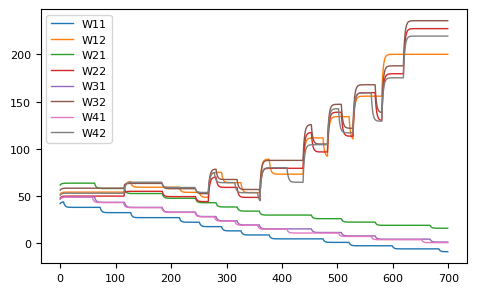
\includegraphics[width=\textwidth]{Figs/ng2-w-r.png}
    \caption{جمعیت نورونی دوم}
  \end{subfigure}
  \caption{نمودار تغییرات وزن‌های سیناپسی جمعیت‌های نورونی}
  \label{Fig:ng1-ng2-w-r}
\end{figure}
\end{center}

\begin{figure}[H]
\centering
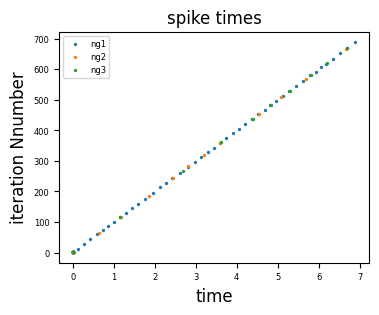
\includegraphics[width=7cm]{Figs/ngs-s-t-r.png}
\caption{زمان ضربه هر سه جمعیت نورونی موجود در شبکه}
\label{Fig:ngs-s-t-r}
\end{figure}
\end{center}

همانطور که در نمودارهای \ref{Fig:ng1-ng2-w-r}
نشان داده شده است در هر دو جمعیت نورونی وزن‌های متصل به خروجی اول به مرور زمان کاهش یافته اند و وزن‌های خروجی به جمعیت دوم افزایش که این رفتار به این دلیل است که دو جمعیت ما کاملا الگوهای مختلفی را به عنوان ورودی می‌گیرند و طبعا انتظار داریم که فعالیت یک از خروجی‌ها بیشتر و دیگری کمتر باشد تا شباهت به کمینه خود برسد و به عبارت دیگر در این نوع یادگیری ما برای یکی از الگو‌ها پاداش می‌دهیم و برای دیگری مجازات می‌کنیم، در نهایت این امر باعث می‌شود که یکی از خروجی‌ها که نشان دهنده فعالیت با پاداش است تقویت شود و دیگری تضعیف می‌شود.


\hfill \break
\subsubsection{تغییرات وزن سیناپسی با ورودی تصادفی پوآسون}

\begin{figure}[H]
\centering
  \begin{subfigure}[b]{0.45\textwidth}
    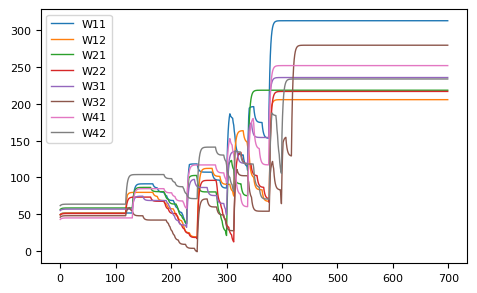
\includegraphics[width=\textwidth]{Figs/w-ng1-r.png}
    \caption{جمعیت نورونی اول با ورودی پرنده}
  \end{subfigure}
  \hspace*{10}
  \begin{subfigure}[b]{0.45\textwidth}
    \includegraphics[width=\textwidth]{Figs/w-ng2-r.png}
    \caption{ جمعیت نورونی دوم با ورودی پل}
  \end{subfigure}
  \caption{نمودار تغییرات وزن‌های سیناپسی جمعیت‌های نورونی}
  \label{Fig:w-ng1-ng2-r}
\end{figure}
\end{center}

\begin{figure}[H]
\centering
\includegraphics[width=7cm]{Figs/ngs-p-s-t-r.png}
\caption{زمان ضربه هر سه جمعیت نورونی موجود در شبکه}
\label{Fig:ngs-p-s-t-r}
\end{figure}
\end{center}

در این آزمایش همانطور که در نمودار‌های \ref{Fig:w-ng1-ng2-r}
مشاهده می‌کنید از آنجایی که هر دو الگو ورودی مشابه هم بودند و از طرفی ما به هر دو ورودی پاداش دادیم و غلظت دوپامین را افزایش دادیم باعث شد که همه وزن‌ها افزایش داشته باشند و خروجی‌های ما الگو های متفاوتی را یاد نمی‌گیرند، می‌توانیم این موضوع را در شباهت کسینوسی نیز مشاهده کنیم.


\hfill \break
\subsection{شباهت کسینوسی}

\subsubsection{شباهت کسینوسی با جریان ثابت نویز دار}

همانطور که بالاتر توضیح دادیم در این قسمت شباهات کسینوسی را در هر مرحله از شبیه سازی محاسبه می‌کنیم که نتیجه آن را  در نمودار \ref{Fig:cos-sim3}	می‌توانید مشاهده کنید. 

\begin{figure}[H]
\centering
\includegraphics[width=6cm]{Figs/cos-sim3.png}
\caption{نمودار  شباهت کسینوسی وزن‌های دو نورون خروجی}
\label{Fig:cos-sim3}
\end{figure}
\end{center}



اگر که وظیفه ما یک $classification$ باشد در آن زمان هر نورون خروجی ما بازنمایی یک کلاس خواهد بود، بنابراین زمانی این مدل به خوبی عمل می‌کند که شباهت میان این نورون‌های خروجی به کمینه خود برسند چون کاملا در این صورت الگوهای متفاوتی را آموخته‌اند، در اینجا هم همانطور که مشاهده می‌کنید به مرور زمان وقتی شبیه سازی را انجام می‌دهیم شباهت میان وزن‌ها کمتر می‌شود که این نشان دهنده یادگیری الگو‌های متفاوت توسط نورون‌های خروجی می‌باشد که این مطابق انتظار ما رفتار خوبی است چونکه ما دوجمعیت با ورودی‌های کاملا متفاوت داشتیم و انتظار داشتیم که بتوانیم تفاوت‌ آن‌ها را در نورون‌های خارجی نیز مشاهده کنیم. در این قسمت با توجه به اینکه به یک الگو پاداش و دیگری مجازات دادیم و کنترل بر یادگیریی داشتیم نسبت به یادگیری \lr{STDP} کاهش بیشتری در شباهت کسینوسی مشاهده می‌کنیم.



\subsubsection{شباهت کسینوسی با ورودی تصادفی پوآسون}
همانطور که ابتدای این بخش توضیح دادیم در این قسمت شباهات کسینوسی را در هر مرحله از شبیه سازی محاسبه می‌کنیم که نتیجه آن را  در نمودار \ref{Fig:cos-sim4}	می‌توانید مشاهده کنید. 


\begin{figure}[H]
\centering
\includegraphics[width=6cm]{Figs/cos-sim4.png}
\caption{نمودار  شباهت کسینوسی وزن‌های دو نورون خروجی}
\label{Fig:cos-sim4}
\end{figure}
\end{center}

اگر که وظیفه ما یک $classification$ باشد وقتی می‌توانیم به خوبی عمل کنیم که شباهت به میزان کمینه خود برسد و این البته در حالتی خوب است که الگو‌های ورودی هم کاملا متفاوت باشند، برای مثال در بخش ورودی با جریان ثابت نویز دار که الگو ها تفاوت زیادی داشتند این شباهت خیلی کم بود و نورون‌های خروجی رفتار های متفاوتی را آموختند اما در این بخش همانطور که در شکل \ref{Fig:cos-sim4}
مشاهده می‌کنید نورون‌های خروجی ما الگو‌های خیلی متفاوتی را نیاموخته‌اند و تقریبا می‌توان گفت که الگو ها با هم مشابه بوده‌اند اما با این حال می‌توان از آن‌ها برای جداسازی کلاس ها استفاده کرد به عبارت دیگر ما به هر دو ورودی در این آزمایش پاداش دادیم و پس الگو‌های خیلی متفاوتی نیاموختند و شباهت زیادی قابل مشاهده است.




\subsection{تاثیر نورون بدون فعالیت}

در این بخش یک جمعیت نورونی با یک نورن به دو جمعیت نورونی ورودی اضافه می‌کنیم که به آن ورودی نمی‌دهیم تا ضربه ای نزند همچنین یک جمعیت نورونی نیز به خروجی اضافه می‌کنیم که در آن نیز با افزایش حد آستانه کاری می‌کنیم که آن نورون ضربه ای نزند، بنابراین در این شبکه جدید نه نورون در لایه ورودی داریم که از سه جمعیت تشکیل شده اند و دو جمعیت در لایه خروجی داریم که در کل سه نورون دارند. 
\subsubsection{تاثیر نورون بدون فعالیت با جریان ورودی ثابت نویزدار}

در این حالت از آنجایی که نورون خروجی‌ای که اضافه کردیم هیچ ضربه ای نمی‌زند بنابراین وزن سیناپسی متصل به آن نورون نیز تغییری ندارد، ما نه نورون متصل به این نورون داریم که تغییرات وزن های سیناپسی را می‌توانید در شکل 
\ref{Fig:out_plus-r}
مشاهده کنید و همانطور که می‌بینید تغییری مشاهده نمی‌شود.

\begin{figure}[H]
\centering
\includegraphics[width=6cm]{Figs/out_plus-r.png}
\caption{تغییر وزن‌های سیناپسی نورون بدون فعالیت خروجی}
\label{Fig:out_plus-r}
\end{figure}
\end{center}


\subsubsection{تاثیر نورون بدون فعالیت با ورودی تصادفی پوآسون}

همانطور که در قسمت قبلی توضیح داده شد از آنجایی که هیچ ضربه ای این نورون خروجی اضافه شده نمی‌زند بنابراین طبق تعریف قانون یادگیری \lr{RSTDP} هیچ تغییری در وزن‌های سیناپسی متصل به این نورون رخ نمی‌دهد و این موضوع را می‌توانید در شکل \ref{Fig:last-w-ch-r} مشاهده کنید.

\begin{figure}[H]
\centering
\includegraphics[width=6cm]{Figs/last-w-ch-r.png}
\caption{تغییر وزن‌های سیناپسی نورون بدون فعالیت خروجی}
\label{Fig:last-w-ch-r}
\end{figure}
\end{center}

\end{document}